
\subsection{Deviation From Put-Call Parity}
The put-call parity relations derived from \textcite{stoll1969relationship} is a classical options pricing concepts in finance. It characterized the relationship that must exist between European put and call options with the identical underlying asset, expiration and strike prices. The equation must hold for European options on no-dividends paying underlying in a perfect market. 
\begin{equation}
C-P = S - PV(K)
\end{equation}
Where C and P represent call prices and put prices, and S is Stock price. With same maturity and exercise price K, the arbitrage opportunity would exist if the equation is not hold. The \textcite{black1973pricing} formula satisfies the put-call parity for any assumed value of the volatility parameter $\sigma$, therefore, 
\begin{equation}
C^{BS}(\sigma ) + PV(K) = P^{BS}(\sigma ) + S
\end{equation}
where $C^{BS}(\sigma )$ and $P^{BS}(\sigma )$ indicate Black-Scholes call and put prices, respectively. 
\\
Combine the above equation, we can derive the equation
\begin{equation}
C^{BS}(\sigma ) - C = P^{BS}(\sigma ) - P
\end{equation}
which implies that the implied volatility of call option and put option should be the same if all equation holds. 
\begin{equation}
IV^{call} = IV^{put}
\end{equation}
Of course the equation may not be hold once the option is American-style. However, our primary studies on SPX option is European style. Therefore, we do not need to consider the dividend payment or early exercise case in our further research. 

Clearly, the larger implied volatilities are the higher the call or put option prices claim. Following \textcite{amin2004index}, we refer to the difference between call and put implied volatilities as the call-put implied volatility spread(CPIV). It is suggested that a positive(negative) CPIV could be viewed as a bullish(bearish) signal regarding the underlying stock. 

The aggregate Intraday CPIV are construced as following steps: 
\begin{enumerate}
\item  We first divided a single day into 14 of 5-minutes interval. Each interval contains the tick data from 2.5 minutes ahead and behind. For example, the 9 a.m. invertal, we collect valid data from 08:47:30 to 09:32:30 to represent this interval. As for open(close) interval, we choose to accumulate the full 5 minutes data behind(ahead)\footnote{We collect the whole transaction data in 5 minutes for trade data. However, the size of quote data is extremely unbalanced in different intervals, we restricted 1000 to 2000 quotes as maximum for call and put in collecting quote data.}

\item Similar to \textcite{xing2010does}, in each interval, we eliminate an option from the sample if its time to expiration is less than 10 days or more than a year, if its open interest is negative, if its moneyness\footnote{Moneyness is defined as the ratio of the strike price to the stock price.} is smaller than 0.9 or more than 1.1. Furthermore, the option quotes must not violate basic no-arbitrage relations.

\item Then, in each time interval, there must be several valid option pairs with identical maturity(T) and exercise price(K). For each option pair we choose only one pair to be the representitive. For quote data, we choose the mean of best bid($\beta ^{\ast }$) best offer($\alpha ^{\ast }$) as the chosen call and put price. For trade data, we capture the transaction that is closet to the centering time.  

\item After collecting several time interval valid option pairs. we calculated the CPIV by applying, 
 \begin{equation}
CPIV_{t} = IV_{t}^{call} - IV_{t}^{put} = \sum_{j = 1}^{N_{t}}\theta _{j,t}(IV_{j,t}^{call} - IV_{j,t}^{put})
 \end{equation}
 
$CPIV_{t}$ denotes the implied volatility spread on interval t; $IV_{j,t}$ describe the B-S implied volatility, where the j refers to valid pairs of put and call options; $\theta_{j,t}$ are weights, there are $N_{t}$ valid pairs of option on interval t. 

Follow by \textcite{holowczak2013aggregating}, the aggregation of option information could be adjusted by the level of moneyness and maturity. 
 \begin{equation}
CPIV_{t} = IV_{t}^{call} - IV_{t}^{put} = \sum_{j = 1}^{N_{t}}w_{j,t}(IV_{j,t}^{call} - IV_{j,t}^{put})
 \end{equation}

The equation is identical except for the weight expression. $w_{j,t}$ is actually $exp(-(m_{j}^{2})/2 -(M_{j} - 1)^{2}) * \theta_{j}$ where $m_{j}^{2}$ measures the moneyness of the option contract.  $m_{j} =  (\frac{K_{i}}{S_{i}} - 1)$ and $K_{i}$ represents exercise prices and $S_{i}$ represents underlying prices; the $M_{j}$ evaluates the maturity of option contract. $M_{j} =  max(1, T_{i}*12) $ and $T_{i}$ represents the maturity in month unit. 


\end{enumerate}


\subsection{Data}
In our analysis, the primary quote and trade intraday data for SPX option originates from CBOE MDR. The sample period studied is from January 2007 to December 2017. The option data includes trade date, trade time, expiration date, put-call code, exercise price, maturities, bid price, ask price, underlying price. The daily price of S\& P 500 index is obtained from Bloomberg. The zero-coupon bond (ZCB) rate represent risk-free rate in B-S formula are collected from WRDS with different duration. The size of the sample data is about 1-TB around and the amount is about 1 billion. After we exclude the tick data fall outside the 5-minutes intervals, it remains about 40 million. Furthermore, we follow the approach from \textcite{ofek2004limited} to exclude the invalid option pairs. Finally, we have 1,692,542 valid volatility spreads for SPX option from January 2007 to December 2017. 


Following the prior studies\textcite{bollerslev2009expected}, several macro-economic variable are suggested to be crucial and informative with regard to future returns. Specifically, we collect data of the default spread(between Moody's BAA and AAA corporate bond spreads), the term spread(between the 10-year T-Bond and 3-month T-bill yields) \footnote{The daily data are collected from the public website of the Federal Reserve Bank of St. Louis.} as control variables in our regression analysis. The set of macro-economics controls used in regressions changes as the measurement window of the expected market returns changes. 


In our study, the amount of intraday CPIV should be 38,668 (14 Intervals * 2,762 Days). However, most of option quote data are short date contract(less than 10 days) in the middle of month so that we have mutiple missing values by this approach. Meanwhile, our research also winsorized the outliers of intraday CPIV on 1\% at the front and end. The final valid interval CPIV of trade data is 36,959, as for quote data is 27,554.


\autoref{table:stats_of_CPIV} presents the descriptive statistics of intraday CPIV.



\begin{table}[h]
\centering
\caption{Descriptive Statistics of Intraday CPIV}\label{table:stats_of_CPIV}
\begin{threeparttable}

\medskip


{\scriptsize 
This table shows descriptive statistics for CPIV of each interval. Panel A presents the summary statsitics for CPIV. Panel B presents the population mean test among CPIV of each interval. In panel A, the first row represents all intervals.  \# Pos.CPIV is the amount of CPIV above zero, where \# Neg.CPIV is the amount of CPIV below zero. Nan Value Rate refers to the rate that CPIV of interval is blank due to the reasons like the option prices are out of boundary, or the maturity are not satisfied with the rules, , etc. In Panel B, the first row and column represent all intervals. the values in the table convey the p-value of population mean test between each interval. 
}
\medskip
\begin{subtable}[t]{\linewidth}

\caption{Panel A: The Descriptive Statistics of CPIV on Quote Data }
\tiny
\begin{tabular}{ccccccccccccccc}
\toprule
\textbf{}        & 08:30 & 09:00 & 09:30 & 10:00 & 10:30 & 11:00 & 11:30 & 12:00 & 12:30 & 13:00 & 13:30 & 14:00 & 14:30 & 15:00 \\ \midrule
Mean(\%)         & -2.45 & -3.73 & -3.65 & -3.59 & -3.57 & -3.57 & -3.62 & -3.61 & -3.60 & -3.62 & -3.62 & -3.58 & -3.51 & -3.41 \\
Std(\%)          & 1.11  & 0.71  & 0.77  & 0.80  & 0.79  & 0.76  & 0.78  & 0.82  & 0.82  & 0.78  & 0.77  & 0.77  & 0.71  & 0.80  \\
Min(\%)          & -51.17 & -14.81 & -11.38 & -14.24 & -10.65 & -10.65 & -11.86 & -11.64 & -13.95 & -11.60 & -10.09 & -14.39 & -11.22 & -15.84 \\
Max(\%)          & 43.20  & 11.69  & 20.39  & 3.49   & 8.91   & 7.09   & 6.52   & 4.38   & 5.21   & 4.92   & 3.51   & 4.22   & 5.62   & 4.67   \\
Median(\%)       & -3.36  & -3.72  & -3.59  & -3.55  & -3.47  & -3.49  & -3.50  & -3.47  & -3.46  & -3.51  & -3.43  & -3.41  & -3.33  & -3.20  \\
\# Pos. CPIV     & 647   & 47    & 24    & 25    & 19    & 22    & 18    & 20    & 19    & 22    & 14    & 19    & 19    & 32    \\
\# Neg. CPIV     & 1916  & 2366  & 2183  & 2099  & 2048  & 1982  & 1943  & 1901  & 1847  & 1802  & 1758  & 1710  & 1649  & 1399  \\
Nan Value Rate(\%) & 3.8   & 9.1   & 16.8  & 19.9  & 22.1  & 24.5  & 26.1  & 27.6  & 29.7  & 31.2  & 33.2  & 34.8  & 37.1  & 46.0  \\ \bottomrule
\end{tabular}
\end{subtable}

\medskip

\begin{subtable}[t]{\linewidth}

\caption{Panel B: The Population Mean Test Among CPIV of Intervals}
\tiny

\begin{tabular}{|c|cccccccccccccc}
\toprule

& 08:30   & 09:00   & 09:30   & 10:00   & 10:30   & 11:00   & 11:30   & 12:00   & 12:30   & 13:00   & 13:30   & 14:00  & 14:30 & 15:00 \\ \midrule
08:30 & 1       &         &         &         &         &         &         &         &         &         &         &        &       &       \\
09:00 & 0.00*** & 1       &         &         &         &         &         &         &         &         &         &        &       &       \\
09:30 & 0.00*** & 0.08*   & 1       &         &         &         &         &         &         &         &         &        &       &       \\
10:00 & 0.00*** & 0.09*   & 0.91    & 1       &         &         &         &         &         &         &         &        &       &       \\
10:30 & 0.00*** & 0.00*** & 0.10    & 0.07*   & 1       &         &         &         &         &         &         &        &       &       \\
11:00 & 0.00*** & 0.00*** & 0.05**  & 0.03**  & 0.77    & 1       &         &         &         &         &         &        &       &       \\
11:30 & 0.00*** & 0.00*** & 0.22    & 0.17    & 0.66    & 0.46    & 1       &         &         &         &         &        &       &       \\
12:00 & 0.00*** & 0.00*** & 0.13    & 0.10    & 0.89    & 0.67    & 0.76    & 1       &         &         &         &        &       &       \\
12:30 & 0.00*** & 0.00*** & 0.06*   & 0.04**  & 0.80    & 0.96    & 0.50    & 0.71    & 1       &         &         &        &       &       \\
13:00 & 0.00*** & 0.00*** & 0.01*** & 0.06*   & 0.93    & 0.84    & 0.61    & 0.83    & 0.87    & 1       &         &        &       &       \\
13:30 & 0.00*** & 0.00*** & 0.00*** & 0.01**  & 0.42    & 0.62    & 0.22    & 0.36    & 0.59    & 0.49    & 1       &        &       &       \\
14:00 & 0.00*** & 0.00*** & 0.00*** & 0.00*** & 0.09    & 0.16    & 0.04**  & 0.07*   & 0.16    & 0.12    & 0.37    & 1      &       &       \\
14:30 & 0.00*** & 0.00*** & 0.00*** & 0.00*** & 0.00*** & 0.00*** & 0.00*** & 0.00*** & 0.00*** & 0.00*** & 0.00*** & 0.04** & 1     &       \\
15:00 & 0.00*** & 0.00*** & 0.00*** & 0.00*** & 0.00*** & 0.00*** & 0.00*** & 0.00*** & 0.00*** & 0.00*** & 0.00*** & 0.00*** & 0.00***& 1   \\
\bottomrule

\end{tabular}

\begin{tablenotes}
%\multicolumn{4}{l}{\footnotesize \textit{Newey-West t} statistics in parentheses} \\
%\multicolumn{4}{l}{\footnotesize * $p < 0.10$, ** $p < 0.05$, *** $p < 0.01$} \\
\item
\item[***]Significant at the 1 percent level.    
\item[**]Significant at the 5 percent level.   
\item[*]Significant at the 10 percent level.
\end{tablenotes}

\end{subtable}
\end{threeparttable}

\end{table}




\subsection{Figure}
\ref{fig:Network}stock trading volume, and stock returns data are taken from CRSP for the construction of control measures.

\begin{figure}[h]
\centering
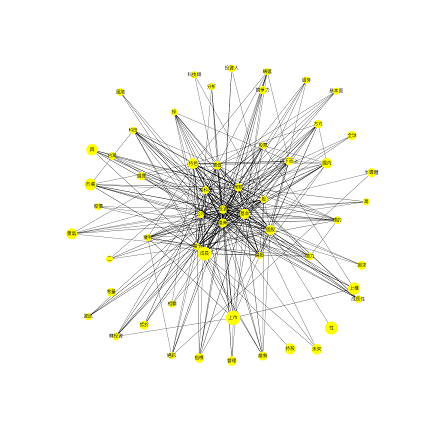
\includegraphics[scale=1.0]{network1}
\caption{Network ot words}
\label{fig:Network}
\end{figure}


\subsection{Variable Definitions}
All measures using implied volatility are calculated using all options with 90 or fewer days to expiration. Following \textcite{cremers2010deviations}, CPIV is the open interest-weighted call implied volatility less open interest weighted put implied volatility. CPIV STD is the standard deviation of CPIV over the past 20 days. IV is the open interest-weighted implied volatility. ME is stock price multiplied by the number of shares outstanding at the end of the measurement period and is reported in billions. Return is the daily, weekly, or monthly return on the day, week, or month, respectively, following CPIV measurement. Reversal is return in the calendar month prior to CPIV measurement. Momentum is the cumulative return in calendar months in brackets relative to the date of CPIV measurement. Turnover is monthly 
volume divided by the number of shares outstanding over calendar months prior to CPIV measurement with months designated in brackets. Illiquidity is the illiquidity measure of Amihud (2002), the absolute value of the return divided by the dollar trading volume averaged over calendar days prior to CPIV measurement, with days designated in brackets.

\subsection{Descriptive Statistics}\label{sec:reganalysis}
This table presents descriptive statistics for xxxx. 
\begin{table}[h]
\centering
\caption{Multivariate Regressions of SPX Return on IVS and Controls -2}
\small
~\\~\\~
\label{Return-2}
\begin{tabular}{@{}cccccccc@{}}
\toprule
                & 12:00      & 12:30      & 13:00      & 13:30      & 14:00      & 14:30      & 15:00      \\ \midrule
Intercept       & 0.00       & 0.00       & 0.00       & 0.00       & 0.00       & 0.00       & 0.00       \\
                & -0.19      & (-0.33)    & -0.84      & -0.50      & -0.16      & -0.35      & -0.09      \\
IVS             & -0.03      & -0.05      & 0.03       & 0.01       & -0.01      & 0.00       & -0.04      \\
                & (-1.08)    & (-1.97)*** & -0.87      & -0.19      & (-0.32)    & (-0.02)    & (-0.81)    \\
DDEF            & 0.00       & 0.00       & 0.00       & 0.00       & 0.00       & 0.00       & 0.00       \\
                & (-0.82)    & (-0.97)    & (-0.55)    & (-0.86)    & (-0.68)    & (-0.74)    & (-1.01)    \\
DTERM           & 0.00       & 0.00       & 0.00       & 0.00       & 0.00       & 0.00       & 0.00       \\
                & -0.54      & -0.96      & -0.99      & -1.21      & -1.02      & -1.10      & -1.14      \\
lag\_return     & -0.10      & -0.10      & -0.10      & -0.10      & -0.10      & -0.11      & -0.10      \\
                & (-3.13)*** & (-3.04)*** & (-3.07)*** & (-3.01)*** & (-2.89)*** & (-3.26)*** & (-3.23)*** \\
                &            &            &            &            &            &            &            \\
Adj Rsquare(\%) & 1.24       & 1.99       & 1.25       & 1.14       & 1.02       & 1.27       & 1.36       \\ \bottomrule
\end{tabular}
\end{table}

